\documentclass[11pt,a4paper]{article}

\usepackage[utf8]{inputenc}
\usepackage[T1]{fontenc}
\usepackage[english]{babel}
\usepackage{lmodern}
\usepackage[margin=2.5cm]{geometry}
\usepackage{amsmath}
\usepackage{array}
\usepackage{booktabs}
\usepackage{float}
\usepackage{caption}
\usepackage{enumitem}
\usepackage{xcolor}
\usepackage{tikz}
\usepackage{microtype}
\usepackage[hidelinks]{hyperref}

\captionsetup{font=small,labelfont=bf}
\setlist{itemsep=2pt,topsep=4pt}
\setlength{\parskip}{4pt}
\renewcommand{\arraystretch}{1.12}

\newcommand{\evidence}[1]{\noindent\textbf{Evidence:} \emph{#1}.\par}
\newcommand{\tests}{\noindent\textbf{Tests.} }
\newcommand{\conclusion}{\noindent\textbf{Conclusion.} }

\title{Continual learning of object detection on the FML Tugger robot\\[4pt]
\large Technical report of the experiments}
\author{Araujo\\Master's thesis, TUM, FML}
\date{November 6, 2026}

\begin{document}
\maketitle

\begin{abstract}
This report describes a system in which a logistics robot learns new object
classes during operation. The robot captures images, SAM3 finds the new class, a
human reviews the uncertain cases, and a single YOLOv8m is retrained to learn the
class without forgetting the old ones. A statistical gate decides whether the
model goes to the robot, which swaps it without restarting. The full cycle worked
once on the real robot, on November 2, 2026: the promoted model detects 7 classes
and loses 2.4\% on the mean of the 5 LOCO classes. This shows that the system is
feasible, not that it is stable: the same configuration passed the gate in 2 of 3
seeds in one round and in 1 of 3 in the repetition. The main findings are:
pseudo-labels from the old model preserve the old classes as well as or better
than human labels; human review gave no measurable improvement on the new class;
202 synthetic images raised the AP of a detector trained from scratch by 12.8\%;
and the gap between environments is the system's largest limit (\texttt{iw\_hub}:
.968 in the lab, .277 on the independent set).
\end{abstract}

\tableofcontents
\newpage

% ---------------------------------------------------------------------------
\section{Goal and conventions}

The goal of the project is to let an intralogistics robot detect objects that
were not in the original training set, with little human work and without losing
what the detector already knew. This combines three problems: annotating images
without a human drawing boxes, adding classes without catastrophic forgetting,
and deciding safely when a new model can go to the robot.

The starting point is a YOLOv8m~\cite{yolov8} trained on LOCO~\cite{loco} with 5
classes: \texttt{small\_load\_carrier} (SLC), \texttt{forklift}, \texttt{pallet},
\texttt{stillage} and \texttt{pallet\_truck}. The system added two classes:
\texttt{iw\_hub}, a yellow robot in the lab, and \texttt{robotic\_arm}, a KUKA
arm.

\paragraph{Conventions.} Unless noted, numbers are AP50 averaged over 3 seeds,
written as in the README (.542 means 0.542). The LOCO classes are measured on
LOCO val: 2277 images from warehouses never seen in training. The reference model
(the ``old model'') has SLC .385, forklift .262, pallet .632, stillage .496 and
pallet\_truck .278, with a mean of .411. Each question in
Section~\ref{sec:questions} states the strength of its evidence: \emph{firm} when
the result repeats across seeds or has a clear confidence interval (CI);
\emph{limited} when there is a small sample, a single seed or a confounder.

% ---------------------------------------------------------------------------
\section{The system}

\subsection{Platforms}

\begin{itemize}
  \item \textbf{Robot (fml-22):} ROS2 Humble, Azure Kinect camera and GTX 1060.
    It runs capture, synchronization, review and inference at 2 Hz.
  \item \textbf{Workstation:} RTX 4090 shared with other users. It runs SAM3,
    training, evaluation and the gate. An hourly cron job executes
    \path{run_pipeline_cycle.py}.
\end{itemize}

\subsection{Data flow}

Figure~\ref{fig:flow} shows the cycle. Images, review decisions and models travel
by rsync over SSH; ROS stays on the robot itself.

\begin{figure}[H]
\centering
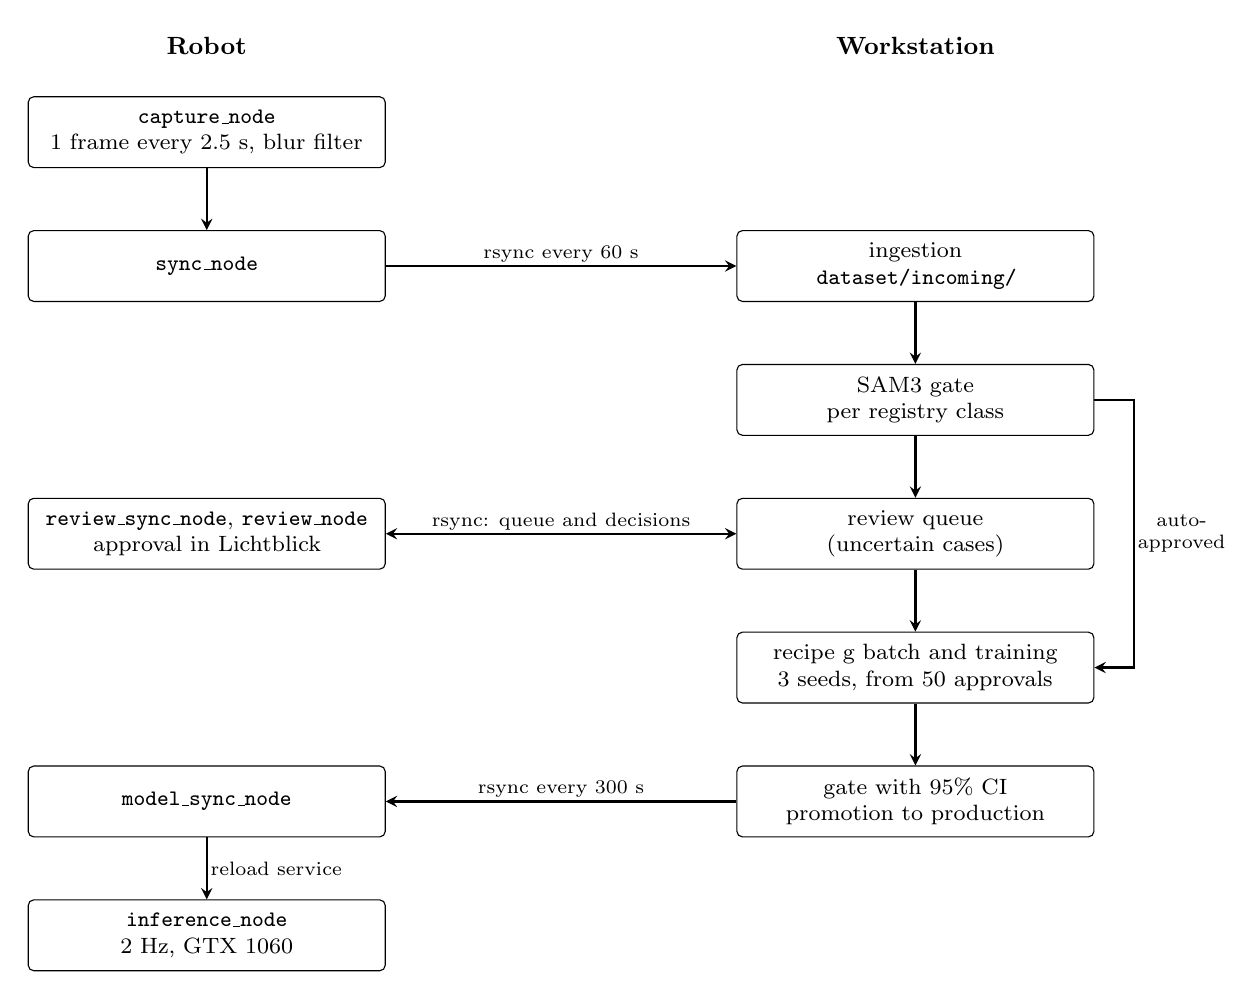
\begin{tikzpicture}[
  font=\footnotesize, >=stealth,
  box/.style={draw, rounded corners=2pt, align=center, minimum height=9mm, text width=43mm},
  arr/.style={->, thick},
  lab/.style={font=\scriptsize, align=center, fill=white, inner sep=1pt}]
  \node[font=\small\bfseries] at (0,1.1) {Robot};
  \node[font=\small\bfseries] at (9,1.1) {Workstation};
  \node[box] (cap) at (0,0)    {\texttt{capture\_node}\\1 frame every 2.5 s, blur filter};
  \node[box] (syn) at (0,-1.7) {\texttt{sync\_node}};
  \node[box] (rev) at (0,-5.1) {\texttt{review\_sync\_node}, \texttt{review\_node}\\approval in Lichtblick};
  \node[box] (mod) at (0,-8.5) {\texttt{model\_sync\_node}};
  \node[box] (inf) at (0,-10.2) {\texttt{inference\_node}\\2 Hz, GTX 1060};
  \node[box] (ing) at (9,-1.7) {ingestion\\\texttt{dataset/incoming/}};
  \node[box] (sam) at (9,-3.4) {SAM3 gate\\per registry class};
  \node[box] (fil) at (9,-5.1) {review queue\\(uncertain cases)};
  \node[box] (tre) at (9,-6.8) {recipe g batch and training\\3 seeds, from 50 approvals};
  \node[box] (gat) at (9,-8.5) {gate with 95\% CI\\promotion to production};
  \draw[arr] (cap) -- (syn);
  \draw[arr] (syn) -- node[lab, above] {rsync every 60 s} (ing);
  \draw[arr] (ing) -- (sam);
  \draw[arr] (sam) -- (fil);
  \draw[arr, <->] (fil) -- node[lab, above] {rsync: queue and decisions} (rev);
  \draw[arr] (fil) -- (tre);
  \draw[arr] (sam.east) -- ++(0.5,0) |- node[lab, pos=0.25, right] {auto-\\approved} (tre.east);
  \draw[arr] (tre) -- (gat);
  \draw[arr] (gat) -- node[lab, above] {rsync every 300 s} (mod);
  \draw[arr] (mod) -- node[lab, right] {reload service} (inf);
\end{tikzpicture}
\caption{Learning cycle between the robot and the workstation.}
\label{fig:flow}
\end{figure}

\subsection{Automatic annotation and human review}

Each new class is defined by a text prompt in \path{class_registry.json}.
SAM3~\cite{sam3} runs on the frames and uses the mean confidence of the boxes: up
to 0.5 the frame is rejected, above 0.5 it passes, and above 0.85 it is approved
automatically. Intermediate cases go to the review queue, where the human only
approves or rejects the frame; boxes are not corrected. Training triggers once
there are at least 50 new approvals.

\subsection{Training recipe}

Each round restarts from the original LOCO model, with \texttt{freeze=21}, imgsz
960, batch 8, 30 fixed epochs, \texttt{last.pt} and 3 seeds. Pseudo-labels always
use confidence 0.5, a decision made on October 7, 2026 together with the decision
to keep a single model. The batch follows recipe g (Table~\ref{tab:recipe}).

\begin{table}[H]
\centering\small
\caption{Composition of the training batch (recipe g).}
\label{tab:recipe}
\begin{tabular}{p{7.2cm}p{7.6cm}}
\toprule
part & labels \\
\midrule
LOCO replay, 10 images per pipeline frame & human \\
Approved frames, up to 150 per class & new classes: SAM3 and review, with the boxes of every class approved in the frame; LOCO classes: old model \\
Copy-paste of the new classes onto LOCO images & inherited \\
Environment frames, rejected by SAM3 for every class & LOCO classes: old model \\
Rest of LOCO train & pseudo-labels per class, as set in the registry: SAM3 or old model \\
\bottomrule
\end{tabular}
\end{table}

\subsection{Promotion gate}

The gate (\path{promote_if_better.py}) compares candidate and production with a
paired bootstrap over the same images, using 1000 resamples. An old class fails
only if the 95\% interval of the difference lies entirely below $-.01$. A new
class needs an AP50 of at least .10 on its first promotion. Among the passing
seeds, the one with the highest mean AP50 is promoted. Before training, a leak
check aborts the batch if it contains any test image.

\subsection{Deployment}

The \texttt{model\_sync\_node} checks production every 300 s, downloads the model,
swaps the file atomically and calls the \texttt{perception/reload\_model} service.
The \texttt{inference\_node} reloads the weights without restarting and publishes
the result on \texttt{/perception/detections\_image}.

% ---------------------------------------------------------------------------
\section{Evaluation methodology}
\label{sec:method}

\begin{itemize}
  \item \textbf{LOCO:} the official split is by warehouse. Train: subsets 2, 3 and
    5. Val: subsets 1 and 4. Val measures generalization to unseen warehouses.
  \item \textbf{iw\_hub:} fixed test set with 30 lab frames, from the same session
    as training, and 50 Roboflow images.
  \item \textbf{robotic\_arm:} 84 frames from October 5 corrected by hand, with
    109 arms. That whole day stays out of training.
  \item \textbf{Noise:} different seeds vary by up to about $\pm.05$ on the weak
    classes. Comparisons therefore use 3 seeds, a fixed batch and a paired CI.
\end{itemize}

\paragraph{Evaluation bugs fixed.} The audit found three problems, and the numbers
from before it were redone or discarded:
\begin{enumerate}
  \item A 0.5 confidence filter before AP, which cut the precision-recall curve.
    The threshold is now 0.001.
  \item An annotation with id 0, which COCOeval treats as unmatched. This pulled
    \texttt{iw\_hub} in the lab down from about 1.0 to .91--.94.
  \item The validation split of the fine-tunes held 170 LOCO val images, which let
    the test set influence checkpoint selection. Clean experiments use 30 fixed
    epochs and \texttt{last.pt}.
\end{enumerate}

% ---------------------------------------------------------------------------
\section{Current results}

\subsection{Captured images}

\begin{table}[H]
\centering\small
\caption{Capture sessions.}
\begin{tabular}{lrp{9.5cm}}
\toprule
session & frames & use \\
\midrule
Sep 16 & 180 & pipeline \\
Sep 17 & 340 & pipeline (iw\_hub and arm training; 30 frames became the iw\_hub test) \\
Oct 5 & 390 & day reserved for testing: never enters training \\
Nov 2, morning & 172 & pipeline (new recording) \\
\textbf{total in pipeline} & \textbf{1082} & \\
Nov 2, afternoon & 391 & outside the pipeline; 88 after removing duplicates; unlabeled \\
\bottomrule
\end{tabular}
\end{table}

\subsection{From captured frame to training: KUKA arm}

\begin{table}[H]
\centering\small
\caption{Funnel of the arm frames, checked against the pipeline database.}
\label{tab:funnel}
\begin{tabular}{p{7cm}rr}
\toprule
stage & with review & without review \\
\midrule
frames analyzed by SAM3 & 1082 & 1082 \\
passed the filter (mean confidence above 0.5) & 221 & 221 \\
after removing the test day (59 frames from Oct 5) & 162 & 162 \\
human decision (161 reviewed, 1 auto-approved) & 116 approved, 46 rejected & none \\
\textbf{in the batch, after removing iw\_hub test images} & \textbf{107} & \textbf{140} \\
\bottomrule
\end{tabular}
\end{table}

Human approval was 72\%. SAM3's mean confidence on the arm stayed between 0.50 and
0.86, so almost nothing was approved automatically. The batch without review
includes 33 frames the human had rejected.

\subsection{Real pipeline round (November 2)}

Round \texttt{pipeline\_finetune\_20261102\_122735} used 190 robot frames (83
iw\_hub and 107 arm). Training the 3 seeds and running the gate took 54 minutes,
from 12:27 to 13:21. The robot downloaded the model at 13:43 and began detecting 7
classes without restarting. The reload call exceeded the 15 s timeout of
\texttt{model\_sync\_node}, but the reload took about 15.5 s on the GTX 1060 and
worked.

\begin{table}[H]
\centering\small
\caption{Real round. The intervals are for the promoted seed against production.}
\label{tab:round}
\begin{tabular}{lrrrrl}
\toprule
class & old & seed 0 (promoted) & seed 1 & seed 2 & 95\% CI of seed 0 \\
\midrule
SLC & .385 & .408 & .403 & .410 & $[+.019,\ +.029]$ \\
forklift & .262 & .225 & .213 & .236 & $[-.078,\ +.010]$ \\
pallet & .632 & .644 & .641 & .644 & $[+.008,\ +.014]$ \\
stillage & .496 & .479 & .470 (fails) & .481 & $[-.029,\ -.006]$ \\
pallet\_truck & .278 & .251 & .261 & .259 & $[-.044,\ -.0097]$ \\
iw\_hub & --- & .549 & .550 & .535 & \\
KUKA arm & --- & .562 & .524 & .520 & \\
\textbf{LOCO mean} & \textbf{.411} & \textbf{.401} & \textbf{.398} & \textbf{.406} & \\
\bottomrule
\end{tabular}
\end{table}

2 of 3 seeds passed. Seed 0 passes on pallet\_truck by a minimal margin: the CI
ends at $-.0097$, and the limit is $-.010$. On the promoted model, \texttt{iw\_hub}
scores .968 on the 30 lab frames and .277 on the 50 Roboflow images. The combined
number (.549) hides this difference; the number that indicates generalization is
.277.

\subsection{Pipeline with and without human review}
\label{sec:review}

The same round was trained twice on a copy of the database. The ``with review''
arm uses the frames approved by the human; the ``without review'' arm uses all
those SAM3 passed. The boxes are the same in both.

\begin{table}[H]
\centering\small
\caption{With and without human review. The last column gives the number of seeds
whose paired CI excludes zero.}
\label{tab:review}
\begin{tabular}{lrrrl}
\toprule
class & old & with review & without review & significant seeds \\
\midrule
\textbf{KUKA arm} & --- & \textbf{.542} & \textbf{.555} & 0 of 3 \\
iw\_hub (lab and Roboflow) & --- & .542 & .592 & 1 of 3, no review better \\
SLC & .385 & .407 & .392 & 3 of 3, no review worse \\
forklift & .262 & .242 & .241 & 0 of 3 \\
pallet & .632 & .644 & .643 & 1 of 3, no review worse \\
stillage & .496 & .476 & .491 & 3 of 3, no review better \\
pallet\_truck & .278 & .253 & .236 & 2 of 3, no review worse \\
\textbf{LOCO mean} & \textbf{.411} & \textbf{.404} & \textbf{.401} & \\
\bottomrule
\end{tabular}
\end{table}

On the arm, seeds were .578 / .545 / .503 with review and .564 / .547 / .553
without. The difference is within noise: the same configuration with review,
trained twice, varied by up to $\pm.02$ per seed (real round .562 / .524 / .520).

\begin{table}[H]
\centering\small
\caption{Gate result against the original LOCO model.}
\label{tab:gate}
\begin{tabular}{lrp{8.4cm}}
\toprule
configuration & passed & failures (95\% CI of the difference) \\
\midrule
\textbf{without review} & \textbf{0 of 3} & pallet\_truck: s0 $[-.063,\ -.028]$, s1 $[-.053,\ -.019]$, s2 $[-.063,\ -.026]$ \\
with review, real round & 2 of 3 & stillage: s1 $[-.037,\ -.015]$ \\
with review, repetition & 1 of 3 & stillage: s0 $[-.033,\ -.011]$, s1 $[-.035,\ -.014]$; pallet\_truck: s1 $[-.050,\ -.016]$ \\
\bottomrule
\end{tabular}
\end{table}

\paragraph{The batches differ in more than the arm frames.} The recipe keeps fixed
proportions, so the 33 extra frames change the whole batch
(Table~\ref{tab:batches}). The batch without review has 36\% fewer pseudo-labeled
LOCO train images, precisely the part that defines recipe g, and more human
replay. The oracle (Section~\ref{q:oracle}) showed that replacing pseudo-labels
with human labels worsens pallet\_truck. The drop in pallet\_truck without review
may therefore come from this change in composition rather than from bad frames.
The experiment does not separate the two causes.

\begin{table}[H]
\centering\small
\caption{Composition of the two batches.}
\label{tab:batches}
\begin{tabular}{lrr}
\toprule
batch part & with review & without review \\
\midrule
robot frames (iw\_hub and arm) & 190 & 223 \\
LOCO replay (train / validation) & 1520 / 380 & 1780 / 450 \\
copy-paste & 738 & 867 \\
environment frames & 503 & 503 \\
LOCO train with pseudo-labels & 920 & 590 \\
\bottomrule
\end{tabular}
\end{table}

\paragraph{Reading.} On the new class, review brought no measurable gain. On the
old classes, no model without review passed the gate, against 3 of 6 with review,
but the sample is small and batch composition is a confounder. The 84 arm test
images were preselected by SAM3 and include no negatives, which may favor training
without review and overestimate AP in both cases.

% ---------------------------------------------------------------------------
\section{Scientific questions, tests and conclusions}
\label{sec:questions}

\subsection{Which zero-shot model works as an automatic annotator?}
\evidence{limited}

\tests Grounding DINO tiny~\cite{gdino}, MM-Grounding-DINO large~\cite{mmgdino},
OWLv2~\cite{owlv2}, LocateAnything-3B (\texttt{nvidia/LocateAnything}) and SAM3 on
LOCO, on samples of 150 images, with prompt and threshold tuning.

\begin{table}[H]
\centering\small
\caption{Zero-shot detectors on LOCO (overall AP50).}
\begin{tabular}{llr}
\toprule
sample & model and configuration & AP50 \\
\midrule
150 images, 4679 boxes & Grounding DINO tiny & .058 \\
& MM-Grounding-DINO large & .000--.008 \\
& OWLv2 base & .125--.143 \\
& SAM3, literal class names & .195 \\
& SAM3, tuned prompts & .408 \\
& SAM3, threshold lowered to 0.2 (many false positives) & .475 \\
\midrule
150 images, seed 42, 4381 boxes & Grounding DINO tiny & .015 \\
& LocateAnything-3B & .101 \\
& SAM3, tuned prompts & .378 \\
\midrule
5097 annotated images (train and val) & SAM3, tuned prompts & .303 \\
\bottomrule
\end{tabular}
\end{table}

\conclusion SAM3 was chosen, with a wide margin over the other models on the same
sample. On the 5097 images, the per-class APs are SLC .369, forklift .261, pallet
.200, stillage .414 and pallet\_truck .272. The comparison is not entirely fair:
SAM3 received more tuning rounds than the others, and the prompt ensemble did not
beat the best single prompt. With few boxes, the sample matters: forklift ranged
from .631 (14 boxes) to .012 (8 boxes) on 150-image samples.

\subsection{How good are SAM3's labels, and where does it fail?}
\evidence{firm}

\tests Comparison with human labels at the operating confidence (0.5) and IoU 0.5,
on two LOCO sets; \texttt{iw\_hub} on 509 Roboflow images; false alarms on 500 LOCO
images; a search for boxes that merge pallets.

\begin{table}[H]
\centering\small
\caption{SAM3 precision and recall against human labels. The sets are different
and should not be mixed.}
\label{tab:sam3q}
\begin{tabular}{lrrrrrr}
\toprule
& \multicolumn{3}{c}{LOCO train (2538 images)} & \multicolumn{3}{c}{LOCO val (2277 images)} \\
\cmidrule(lr){2-4}\cmidrule(lr){5-7}
class & precision & recall & boxes & precision & recall & boxes \\
\midrule
SLC & .45 & .36 & 11956 & .59 & .65 & 8911 \\
forklift & .31 & .56 & 438 & .09 & .31 & 124 \\
pallet & .45 & .26 & 61066 & .54 & .32 & 52297 \\
stillage & .58 & .44 & 3149 & .60 & .56 & 2007 \\
pallet\_truck & .57 & .33 & 1531 & .76 & .38 & 1153 \\
\bottomrule
\end{tabular}
\end{table}

\conclusion SAM3 is excellent on a single, distinct object: on \texttt{iw\_hub},
precision .99, recall .73, mean IoU .88 and no false box in 500 LOCO images. In the
gate, the 509 images would split into 244 auto-approved, 128 for review and 137
rejected. On the arm, against the corrected test set, precision is about .98 and
recall about .80. In dense scenes it is weak. On pallet, 634 boxes merge stacked or
adjacent pallets, in 459 of the 2191 images with 4 or more pallets (21\%).

\subsection{Does a detector trained without human labels approach one trained with them?}
\evidence{firm}

\tests YOLOv8m trained from \texttt{yolov8m.pt}, imgsz 960, batch 16, 150 epochs,
patience 40 and \texttt{best.pt}, 3 seeds. Same images (2538 train, 282
validation), swapping human labels for SAM3 labels at 0.5. Tested on LOCO val with
human labels.

\begin{table}[H]
\centering\small
\caption{Training from scratch with human and SAM3 labels.}
\begin{tabular}{lrrl}
\toprule
class & human & SAM3 & seeds with a significant difference \\
\midrule
SLC & .349 & \textbf{.427} & 3 of 3, SAM3 better \\
forklift & \textbf{.125} & .078 & 2 of 3, SAM3 worse \\
pallet & \textbf{.616} & .319 & 3 of 3, SAM3 worse \\
stillage & .421 & .437 & 0 of 3 \\
pallet\_truck & .173 & \textbf{.213} & 2 of 3, SAM3 better \\
\textbf{mean} & \textbf{.337} & \textbf{.295} & seeds: .318 / .342 / .351 and .291 / .310 / .283 \\
\bottomrule
\end{tabular}
\end{table}

\conclusion The model without human labels reaches 88\% of the one with them.
Pallet explains almost the entire loss; without that class, the mean is .289 for
SAM3 and .267 for humans. The human models fall below production because
production chose its \texttt{best.pt} on LOCO val itself, while here validation is
separate from the test set.

\subsection{Do generic techniques prevent forgetting when a class is added?}
\evidence{limited}

\tests BatchNorm freezing, stratified replay, native distillation, per-class
weighting, copy-paste~\cite{copypaste}, fewer frozen layers, gradient masking,
joint training and YOLOv8l. One seed per candidate.

\begin{table}[H]
\centering\small
\caption{Generic techniques (one seed; differences below .05 on the weak classes
are within noise).}
\begin{tabular}{lrrrr}
\toprule
class & old & copy-paste & joint training & YOLOv8l \\
\midrule
SLC & .385 & .376 & .365 & .451 \\
forklift & .262 & .183 ($-30\%$) & .175 ($-33\%$) & .179 ($-32\%$) \\
pallet & .632 & .637 & .631 & .637 \\
stillage & .496 & .459 & .474 & .556 \\
pallet\_truck & .278 & .206 ($-26\%$) & .211 ($-24\%$) & .233 ($-16\%$) \\
iw\_hub (lab / Roboflow) & --- & .997 / .421 & .990 / .338 & 1.000 / .311 \\
\bottomrule
\end{tabular}
\end{table}

\conclusion None solves it. Gradient masking makes everything worse, because the
LOCO classifier drifts out of alignment with the shared features, which keep
changing. Even joint training, with almost all of annotated LOCO, regresses
forklift and pallet\_truck, which suggests the problem is not only a lack of
replay. YOLOv8l improves SLC and stillage, but it is compared to a YOLOv8m
production model.

\subsection{Which single-model recipe best preserves the old classes?}
\evidence{firm}

\tests Eight variants under the same protocol, 3 seeds. Before that,
self-training rounds along the lines of Mayershofer et al.~\cite{selftraining},
with the student and with production as teacher, and adaptive thresholds along the
lines of Song et al.~\cite{apple}.

\begin{table}[H]
\centering\small
\caption{Fine-tune variants when adding iw\_hub. The loss is of the LOCO mean
against the old model, recomputed from the raw files; iw\_hub is the AP50 on the 50
Roboflow images.}
\label{tab:baselines}
\setlength{\tabcolsep}{4pt}
\begin{tabular}{lrrrrrrrr}
\toprule
variant & SLC & fork. & pallet & still. & p.\_truck & mean & loss & iw\_hub \\
\midrule
a naive & .150 & .000 & .197 & .156 & .000 & .101 & $-75.5\%$ & .363 \\
b replay & .380 & .131 & .639 & .450 & .205 & .361 & $-12.0\%$ & .344 \\
c replay and distillation & .379 & .179 & .640 & .456 & .225 & .376 & $-8.4\%$ & .344 \\
d copy-paste & .375 & .142 & .638 & .446 & .203 & .361 & $-12.1\%$ & .313 \\
e self-training & .372 & .204 & .635 & .451 & .212 & .375 & $-8.7\%$ & .250 \\
f hybrid bank & .373 & .230 & .632 & .458 & .240 & .386 & $-5.9\%$ & .327 \\
\textbf{g pseudo-labels} & .386 & .220 & .636 & .462 & .270 & \textbf{.395} & $\mathbf{-3.9\%}$ & .269 \\
h joint training & .373 & .175 & .646 & .465 & .216 & .375 & $-8.7\%$ & .374 \\
\bottomrule
\end{tabular}
\end{table}

\conclusion Recipe g is the best for the old classes. On the 30 lab frames,
\texttt{iw\_hub} stays at .98--1.0 in every variant. In this test, no single-model
variant passed the gate.

The self-training rounds showed that the teacher matters. With the student as
teacher, pallet\_truck fell from .220 to .190 and that class's labels shrank from
55 to 30 to 19 across rounds: forgetting amplifies itself. With production as
teacher, forklift stayed at .256 and pallet\_truck at .216, and extra rounds added
nothing. Adaptive thresholds raised pallet\_truck (.242 to .252) but dropped
stillage (.465 to .446) and forklift (.253 to .214), with a LOCO mean of .386, and
were discarded.

\subsection{Does forgetting come from bad labels?}
\label{q:oracle}
\evidence{firm}

\tests Oracle: the same 1760 LOCO train images and the same recipe, replacing
pseudo-labels with human labels on stillage and pallet\_truck, and then on all
classes. 3 seeds.

\begin{table}[H]
\centering\small
\caption{Oracle annotator.}
\begin{tabular}{lrrrrrr}
\toprule
arm & SLC & forklift & pallet & stillage & pallet\_truck & mean \\
\midrule
pseudo-labels & .391 & .233 & .637 & .469 & \textbf{.261} & \textbf{.398} \\
human on stillage and pallet\_truck & .393 & .254 & .637 & .465 & .222 & .394 \\
human on all classes & .368 & .199 & .645 & .474 & .221 & .382 \\
\bottomrule
\end{tabular}
\end{table}

\conclusion No. Human labels do not reduce forgetting, and pallet\_truck gets worse
even with more boxes (1002 against 589 in the batch). The proposed interpretation
is that pseudo-labels from the old model act as distillation~\cite{hinton}: the new
model imitates the old one, errors included. This is the most original finding of
the work, but the mechanism was inferred, not tested directly.

\subsection{Does isolating the new class in a second model prevent forgetting?}
\evidence{firm}

\tests Intact LOCO model plus a YOLOv8s specialist, in the style of parameter
isolation~\cite{progressive}, with a false-positive gate of at most 1\% of LOCO
images. 3 seeds.

\conclusion It does so by construction: the LOCO classes stay identical. The cost
is 57 ms per frame on the robot, against 38 ms for the model alone. It passes in 2
of 3 seeds, with false-positive rates of 0.18\%, 2.06\% and 0.35\%; seed 1 fails.
The approach was dropped on October 7 by the decision to keep a single model.

\subsection{How many classes can the single model handle?}
\evidence{limited}

\tests Incremental addition of up to 70 COCO~\cite{coco} classes (excluding
\texttt{person}), with 300 training and 200 evaluation images per class.

\begin{table}[H]
\centering\small
\caption{Mean AP50 per fixed group of classes in the saturation test.}
\begin{tabular}{lrrrrr}
\toprule
group & right after learning & 20 classes & 40 classes & 70 classes & loss \\
\midrule
1--10 & .112 & .098 & .082 & .079 & $-29\%$ \\
11--20 & .123 & --- & .116 & .103 & $-16\%$ \\
21--40 & .078 & --- & --- & .072 & $-7\%$ \\
\bottomrule
\end{tabular}
\end{table}

\conclusion The decline of the first group almost stops between 40 and 70 classes.
LOCO falls from .411 to .364 with 40 classes ($-11\%$). Absolute AP is low (11 of
the 70 classes below .01), so the test measures a trend, not a model that is good
at each class.

\subsection{How can we reliably decide whether a model can be deployed?}
\evidence{firm}

\tests Evaluation audit (Section~\ref{sec:method}); gate with paired bootstrap and
95\% CI; leak check.

\conclusion A fixed tolerance of $-.01$ is smaller than the noise between seeds; the
CI solves this. Two real leaks appeared:
\begin{itemize}
  \item An image bank drawn from all 5 warehouses, including the 2 validation ones,
    gave a mean of .491, a false +19\%. Redone with the training warehouses only,
    the same method gave .393. This case motivated the leak check.
  \item In the real round, 9 frames approved for the arm were iw\_hub test images.
    The leak check blocked the first attempt, and test images of any class are now
    excluded.
\end{itemize}

\subsection{Does the system learn a second class without forgetting the first?}
\evidence{limited}

\tests KUKA arm, 3 seeds, with the same 84-image test set. First offline, from seed
2 of recipe g and without review (120 frames with the arm, 199 boxes). Then, in the
real round, from the original LOCO model.

\begin{table}[H]
\centering\small
\caption{Second class: offline experiment and real round.}
\begin{tabular}{lrrr}
\toprule
class & base (g, seed 2) & offline, with arm & real round (mean of 3 seeds) \\
\midrule
SLC & .384 & .399 & .407 \\
forklift & .229 & .226 & .225 \\
pallet & .636 & .635 & .643 \\
stillage & .463 & .462 & .477 \\
pallet\_truck & .272 & .237 & .257 \\
iw\_hub & .531 & .584 & .545 \\
KUKA arm & --- & .305 & .535 \\
gate & --- & 0 of 3 & 2 of 3 \\
\bottomrule
\end{tabular}
\end{table}

\conclusion The arm went from .305 to .52--.56. The two configurations differ in
several ways: starting model, review, new recording and per-frame label merging.
The cause of the gain was therefore not isolated, and the offline gate used a
different reference (the base itself). The test comes from the same environment as
training and was preselected by SAM3.

\subsection{Does the full cycle work end to end on the real robot?}
\evidence{limited}

\tests Real round on November 2: teleoperated recording (172 frames, from 10:45 to
10:52), SAM3, review, training, gate, promotion, download by the robot and live
inference. The demonstration was recorded on video.

\conclusion Yes, once. It was the first promotion since the initial model, with a
minimal margin on pallet\_truck and 2 of 3 seeds; the repetition of the same
configuration passed in 1 of 3. This shows feasibility, not stability over several
rounds.

\subsection{How much does human review add for a new class?}
\evidence{limited}

\tests The same round with the 107 approved frames and with the 140 frames SAM3
passed, 3 seeds, paired CI (Section~\ref{sec:review}).

\conclusion No measurable gain on the arm (.542 against .555, 0 of 3 seeds). Without
review, 0 of 3 models pass the gate, all because of pallet\_truck, against 3 of 6
with review. Review may protect the old classes, but the sample is small and the
batches also differ in composition, including 920 against 590 pseudo-labeled images.
The result holds for review that only filters frames and for this test set,
preselected by SAM3.

\subsection{Do synthetic images improve detection on real images?}
\evidence{firm}

\tests Human LOCO labels plus 202 Isaac Sim~\cite{isaac} renders (7.4\% of the 2740
training images), 3 seeds, with validation and test on real images only. The renders
hold 97 SLC, 123 forklift, 70 pallet, 94 stillage and 104 pallet\_truck boxes. A
first round lost the pallet labels through a class-mapping error and was redone; it
had given a mean of .362.

\begin{table}[H]
\centering\small
\caption{Training from scratch with and without synthetic images.}
\begin{tabular}{lrrrl}
\toprule
class & human & with synthetic & gain & seeds with a significant difference \\
\midrule
SLC & .349 & .380 & $+9\%$ & 2 of 3 better, 1 no difference \\
forklift & .125 & \textbf{.221} & $+77\%$ & 2 of 3 better, 1 no difference \\
pallet & .616 & .622 & $+1\%$ & 2 of 3 better, 1 of 3 worse \\
stillage & .421 & .463 & $+10\%$ & 3 of 3 better \\
pallet\_truck & .173 & .216 & $+25\%$ & 3 of 3 better \\
\textbf{mean} & \textbf{.337} & \textbf{.380} & $+12.8\%$ & seeds: .362 / .384 / .395 \\
\bottomrule
\end{tabular}
\end{table}

\conclusion Yes, and no class gets consistently worse. The largest gain comes from
the rarest class: forklift has 438 real boxes, and the synthetic set adds 123. This
holds for training from scratch and a single proportion. Forklift varies a lot
between seeds (.142 to .309). It has not yet been tested inside the continual
pipeline.

\subsection{Does what the robot learns generalize beyond its environment?}
\evidence{firm}

\tests \texttt{iw\_hub} on 30 lab frames against 50 Roboflow images; an image bank
from the test warehouses against one from the training warehouses; val against test
in training from scratch.

\conclusion Only a little. \texttt{iw\_hub} falls from .968 to .277. The same method
gives .491 with images from the test warehouses and .393 with other warehouses. In
training from scratch, mAP50 falls from about .77 on val to about .30--.38 on the
test set. The gap between environments is the system's main limit.

\subsection{Can a vision-language model replace the annotator?}
\evidence{limited}

\tests Claude Opus 5.5 annotating 26 LOCO val images by hand, with a coordinate
grid, against human labels at IoU 0.5. The test was stopped before the 100 planned
images.

\begin{table}[H]
\centering\small
\caption{Vision-language model as annotator.}
\begin{tabular}{lrrrrr}
\toprule
class & human boxes & model boxes & hits & precision & recall \\
\midrule
pallet & 889 & 198 & 76 & .38 & .09 \\
pallet\_truck & 5 & 6 & 4 & .67 & .80 \\
\bottomrule
\end{tabular}
\end{table}

\conclusion Not for dense scenes. LOCO has about 34 pallets per image, 71\% of them
on high shelves, and almost none of those were annotated. Of the 198 boxes, 65 had
an IoU between 0.3 and 0.5: right object, imprecise box. Pallet\_truck does well, but
with only 5 boxes. The 6 images used to learn the conventions are included in these
numbers. Use as a box reviewer was not tested.

\subsection{Does the recipe work on an external benchmark?}
\evidence{limited}

\tests CUB~\cite{cub}, Incremental Zero-Shot Learning protocol of Wei et
al.~\cite{izsl}: standard ZSL split, 5 stages of 30 classes, SAM3 for the 50 unseen
classes.

\begin{table}[H]
\centering\small
\caption{CUB: unseen classes (u), seen classes (s) and harmonic mean (H).}
\begin{tabular}{llrrr}
\toprule
method & keeps old images? & u & s & H \\
\midrule
Wei et al. & no & 38.1 & 45.6 & 41.5 \\
ours, no replay & no & 33.4 & 13.7 & 19.5 \\
ours, 5 images per class & 5 per class & 44.7 & 26.0 & 32.9 \\
ours, full replay & all & 44.1 & 46.3 & 45.2 \\
joint training (paper's ceiling) & all & 43.7 & 57.7 & 49.7 \\
\bottomrule
\end{tabular}
\end{table}

\conclusion With full replay, H is above the paper; without replay, the method
collapses. It depends on keeping old data, which the paper does not do, and SAM3's
pretraining may include these species. It suits the scenario in which the old
dataset remains available.

% ---------------------------------------------------------------------------
\section{Limitations and open items}

\begin{itemize}
  \item Only 3 seeds, a single robot environment and a single real round.
  \item Passing the gate is close to the limit and varies between repetitions.
  \item Arm test set: 84 images from the same environment, preselected by SAM3 and
    without negatives.
  \item \texttt{iw\_hub} test set: only 50 Roboflow images. This is a public
    third-party set from 2024, and its origin needs to be confirmed
    (Appendix~\ref{ap:notes}). The November 2 afternoon recording remains unlabeled.
  \item Many near-duplicate frames: in the afternoon recording, 391 became 88.
  \item The review ablation does not isolate frame quality: batch composition also
    changes.
  \item The distillation mechanism was inferred, not tested. Protecting pallet\_truck
    remains open.
  \item Synthetic data has not yet been tested inside the pipeline.
  \item TUM rules on declaring AI use: check before submission.
\end{itemize}

% ---------------------------------------------------------------------------
\appendix

\section{Data verification notes}
\label{ap:notes}

While preparing this report, the numbers were checked against the raw files and the
pipeline database. The points below differ from the README or the experiment log,
and the version given here prevails.

\begin{enumerate}
  \item \textbf{SAM3 ``on the full val'' (.30).} The value .303 comes from 5097
    images, which corresponds to train (2820) and val (2277) combined, not val alone.
  \item \textbf{Difference in \path{sam3_label_quality.json}.} This file measures LOCO
    val; the README table measures LOCO train. They are different sets, and
    Table~\ref{tab:sam3q} gives both. The exact cause of the difference was not
    investigated.
  \item \textbf{Held-out frames from October 5.} The database has 59 arm frames
    marked \texttt{held\_out\_test}, which closes the count 221 $-$ 59 = 162. The
    experiment log said 74.
  \item \textbf{Loss of recipe g.} Recomputed, it is $-3.9\%$, not $-3.8\%$.
  \item \textbf{Review confounder.} The README mentions the difference in the number
    of frames, but not batch composition (Table~\ref{tab:batches}).
  \item \textbf{SAM3 forklift (.012).} This comes from a sample with only 8 boxes; on
    the 5097 images the value is .261.
  \item \textbf{Roboflow origin.} The README treats the set as independent, but the
    docstring of \path{sam3_label_quality.py} says it comes from the robot's lab. The
    dataset page confirms neither. If it comes from the same lab, .277 measures
    another session, not another environment.
  \item \textbf{Pipeline README.} \path{dataset/pipeline/README.md} still describes
    the 5000-image bank and says rounds do not promote; both points are out of date.
\end{enumerate}

\section{Where the data is}

\begin{table}[H]
\centering\small
\caption{Results and scripts of each experiment, in \texttt{dataset/pipeline/}.}
\begin{tabular}{p{3.6cm}p{4.6cm}p{6.6cm}}
\toprule
experiment & script & results \\
\midrule
Recipe variants & \path{baselines.py} & \path{self_training/results_baselines.json} \\
Oracle & \path{oracle_annotator.py} & \path{self_training/results_oracle_annotator.json} \\
SAM3 quality & \path{sam3_label_quality.py} & \path{sam3_label_quality.json} \\
SAM3 against human & \path{loco_sam3_vs_human.py} & \path{self_training/results_loco_sam3_vs_human.json} \\
Synthetic & \path{loco_synthetic_mix.py} & \path{self_training/results_loco_synthetic_mix.json} \\
Offline arm & \path{kuka_arm_experiment.py} & \path{self_training/results_kuka_arm.json} \\
Real round & \path{run_pipeline_cycle.py} & \path{self_training/results_pipeline_round_20261102.json} \\
With and without review & \path{kuka_review_ablation.py} & \path{self_training/results_kuka_review_ablation.json} and \path{_gate.json} \\
Zero-shot detectors & \path{eval_loco.py} (in \texttt{dataset/}) & \path{dataset/results/loco_eval_results_zeroshot.csv} \\
\bottomrule
\end{tabular}
\end{table}

\begin{thebibliography}{99}
\bibitem{loco} C.~Mayershofer, D.-M.~Holm, B.~Molter and J.~Fottner.
  LOCO: Logistics Objects in Context. \emph{IEEE ICMLA}, 2020.
\bibitem{yolov8} G.~Jocher, A.~Chaurasia and J.~Qiu. Ultralytics YOLOv8. Software, 2023.
\bibitem{sam3} N.~Carion et al. SAM 3: Segment Anything with Concepts. 2025.
\bibitem{gdino} S.~Liu et al. Grounding DINO: Marrying DINO with Grounded
  Pre-Training for Open-Set Object Detection. \emph{ECCV}, 2024.
\bibitem{mmgdino} X.~Zhao et al. An Open and Comprehensive Pipeline for Unified
  Object Grounding and Detection. 2024.
\bibitem{owlv2} M.~Minderer, A.~Gritsenko and N.~Houlsby. Scaling Open-Vocabulary
  Object Detection. \emph{NeurIPS}, 2023.
\bibitem{selftraining} C.~Mayershofer, T.~Fischer and J.~Fottner. Improving visual
  object detection using synthetic self-training. \emph{Logistics Journal}, 2021.
\bibitem{apple} Song et al. Overcoming Catastrophic Forgetting for Multi-Label
  Class-Incremental Learning. \emph{WACV}, 2024.
\bibitem{izsl} K.~Wei, C.~Deng, X.~Yang and D.~Tao. Incremental Zero-Shot Learning.
  \emph{IEEE Transactions on Cybernetics}, 2022.
\bibitem{hinton} G.~Hinton, O.~Vinyals and J.~Dean. Distilling the Knowledge in a
  Neural Network. 2015.
\bibitem{progressive} A.~Rusu et al. Progressive Neural Networks. 2016.
\bibitem{copypaste} G.~Ghiasi et al. Simple Copy-Paste is a Strong Data
  Augmentation Method for Instance Segmentation. \emph{CVPR}, 2021.
\bibitem{coco} T.-Y.~Lin et al. Microsoft COCO: Common Objects in Context.
  \emph{ECCV}, 2014.
\bibitem{cub} C.~Wah et al. The Caltech-UCSD Birds-200-2011 Dataset. Technical
  report, Caltech, 2011.
\bibitem{isaac} NVIDIA. Isaac Sim. Software.
\end{thebibliography}

\end{document}
